\documentclass[hidelinks,12pt]{article}
\usepackage[left=0.25cm,top=1cm,right=0.25cm,bottom=1cm]{geometry}
%\usepackage[landscape]{geometry}
\textwidth = 20cm
\hoffset = -1cm
\usepackage[utf8]{inputenc}
\usepackage[spanish,es-tabla]{babel}
\usepackage[autostyle,spanish=mexican]{csquotes}
\usepackage[tbtags]{amsmath}
\usepackage{nccmath}
\usepackage{amsthm}
\usepackage{amssymb}
\usepackage{mathrsfs}
\usepackage{graphicx}
\usepackage{subfig}
\usepackage{standalone}
\usepackage[outdir=./Imagenes/]{epstopdf}
\usepackage{siunitx}
\usepackage{physics}
\usepackage{color}
\usepackage{float}
\usepackage{hyperref}
\usepackage{multicol}
%\usepackage{milista}
\usepackage{anyfontsize}
\usepackage{anysize}
%\usepackage{enumerate}
\usepackage[shortlabels]{enumitem}
\usepackage{capt-of}
\usepackage{bm}
\usepackage{relsize}
\usepackage{placeins}
\usepackage{empheq}
\usepackage{cancel}
\usepackage{wrapfig}
\usepackage[flushleft]{threeparttable}
\usepackage{makecell}
\usepackage{fancyhdr}
\usepackage{tikz}
\usepackage{bigints}
\usepackage{scalerel}
\usepackage{pgfplots}
\usepackage{pdflscape}
\pgfplotsset{compat=1.16}
\spanishdecimal{.}
\renewcommand{\baselinestretch}{1.5} 
\renewcommand\labelenumii{\theenumi.{\arabic{enumii}})}
\newcommand{\ptilde}[1]{\ensuremath{{#1}^{\prime}}}
\newcommand{\stilde}[1]{\ensuremath{{#1}^{\prime \prime}}}
\newcommand{\ttilde}[1]{\ensuremath{{#1}^{\prime \prime \prime}}}
\newcommand{\ntilde}[2]{\ensuremath{{#1}^{(#2)}}}

\newtheorem{defi}{{\it Definición}}[section]
\newtheorem{teo}{{\it Teorema}}[section]
\newtheorem{ejemplo}{{\it Ejemplo}}[section]
\newtheorem{propiedad}{{\it Propiedad}}[section]
\newtheorem{lema}{{\it Lema}}[section]
\newtheorem{cor}{Corolario}
\newtheorem{ejer}{Ejercicio}[section]

\newlist{milista}{enumerate}{2}
\setlist[milista,1]{label=\arabic*)}
\setlist[milista,2]{label=\arabic{milistai}.\arabic*)}
\newlength{\depthofsumsign}
\setlength{\depthofsumsign}{\depthof{$\sum$}}
\newcommand{\nsum}[1][1.4]{% only for \displaystyle
    \mathop{%
        \raisebox
            {-#1\depthofsumsign+1\depthofsumsign}
            {\scalebox
                {#1}
                {$\displaystyle\sum$}%
            }
    }
}
\def\scaleint#1{\vcenter{\hbox{\scaleto[3ex]{\displaystyle\int}{#1}}}}
\def\bs{\mkern-12mu}


\title{Introducción a las Ecuaciones Diferenciales Parciales \\[0.3em]  \large{Tema 2 - Primeras técnicas de solución} \vspace{-3ex}}
\author{M. en C. Gustavo Contreras Mayén}
\date{ }

\pagestyle{fancy}
\fancyhf{}
\rhead{Curso MAF}
\lhead{\leftmark}
\rfoot{\thepage}
\setlength{\headheight}{16pt}%

\begin{document}
\vspace{-4cm}
\maketitle
\fontsize{14}{14}\selectfont
\tableofcontents
\newpage

\section{Método de separación de variables.}

El método de separación de variables es una de las técnicas más antiguas para resolver problemas de valores con condiciones iniciales y se aplica en problemas donde:
\begin{enumerate}
\item La EDP es lineal y homogénea (no necesariamente con coeficientes constantes).
\item Las condiciones de frontera tienen la forma:
\begin{align*}
\alpha \, u_{x} (0, t) + \beta \, u(0, t) &= 0 \\
\gamma \, u_{x} (1, t) + \delta \, u(1, t) &= 0
\end{align*}
donde $\alpha, \beta, \gamma, \delta$ son constantes (las condiciones de frontera de esta forma se denominan \textbf{condiciones de frontera lineales homogéneas}).
\end{enumerate}

Como referencia histórica, este método se remonta a la época de Joseph Fourier (de hecho, ocasionalmente se le llama \emph{método de Fourier}) y es probablemente el método de solución más utilizado (cuando corresponde).
\par
En lugar de mostrar cómo funciona el método en general, apliquémoslo a un problema específico.

\subsection{Planteamiento del problema.}

Considera el siguiente problema de valores iniciales con la ecuación de calor:
\\
Ecuación diferencial:
\begin{align*}
\addtolength{\fboxsep}{5pt}\boxed{ u_{t} = \alpha^{2} \, u_{xx}, \hspace{1.5cm} 0 < x < L,\hspace{0.5cm} 0 < t < \infty}
\end{align*}

Con las condiciones de frontera (CDF):
\begin{align*}
\addtolength{\fboxsep}{5pt}\boxed{
\begin{cases}
u(0, t) = 0 \\
u(L, t) = 0
\end{cases}
\hspace{1.5cm}
0 < t < \infty }
\end{align*}

Y las condiciones iniciales (CI):
\begin{align*}
\addtolength{\fboxsep}{5pt}\boxed{
u(x, 0) = \phi (x) \hspace{1.5cm} 0 \leq x \leq L
}
\end{align*}

Antes de revisar el método de separación de variables, pensemos primero en nuestro problema: Aquí tenemos una varilla finita de longitud $L$ donde la temperatura en los extremos se fija en cero (supongamos que es un problema de temperatura donde cero significa tantos grados). 
\begin{figure}[H]
    \centering
    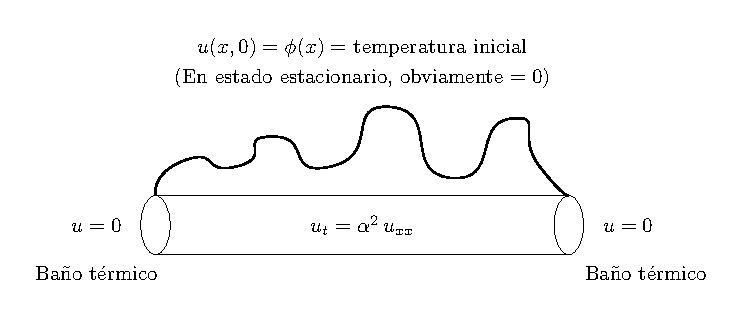
\includegraphics[scale=1.3]{Imagenes/Separacion_Variables_00_Barra.eps}
    \caption{Esquema que representa la barra conductora así como las condiciones iniciales y de frontera.}
    \label{fig:figura_barra_01}
\end{figure}

También se nos dan datos sobre el problema en forma de condición inicial; nuestro objetivo es encontrar la temperatura $u (x, t)$ en puntos posteriores en el tiempo.

Ahora veamos una descripción general.

\subsection{La técnica.}

El método de separación de variables supone la existencia de soluciones sencillas de una EDP de la forma:
\begin{align*}
u(x, t) =  X(x) \, T(t)
\end{align*}

donde $X (x)$ es alguna \emph{función que depende solo de} $x$ y $T (t)$ es alguna \emph{función que depende solo de} $t$.
\par
Las soluciones son sencillas porque cualquier temperatura $u (x, t)$ de esta forma conservará su \enquote{forma} básica para diferentes valores de tiempo $t$, como podemos ver en la figura (\ref{fig:figura_separacion_variables_01})
\begin{figure}[H]
    \centering
    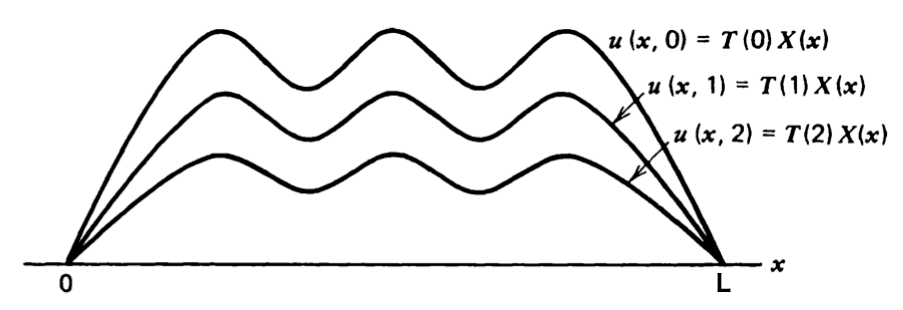
\includegraphics[scale=0.4]{Imagenes/Separacion_Variables_01.png}
    \caption{Gráfica de $X(x)$ y $T(t)$ para distintos valores de $t$.}
    \label{fig:figura_separacion_variables_01}
\end{figure}

La idea general que tenemos nos plantea la posibilidad de encontrar un número infinito de estas soluciones a la EDP (que al mismo tiempo también satisfacen las condiciones de frontera). Estas funciones simples son:
\begin{align*}
u_{n} (x, t) = X_{n} (x) \, T_{n}(t)
\end{align*}

se les denomina \textbf{soluciones fundamentales}, son las componentes básicas de nuestro problema, y de la solución $u (x, t)$ que estamos buscando. Sumando las soluciones fundamentales $X_{n}(x) \, T_{n} (t)$ de tal manera que la suma resultante
\begin{align*}
\sum_{n=1}^{\infty} A_{n} \, X_{n} (x) \, T_{n} (t)
\end{align*}

satisface las condiciones iniciales. Dado que esta suma aún satisface la EDP y las CDF, ahora tenemos la solución a nuestro problema. Veamos a detalle el método de separación de variables.

\subsection{Paso 1.}

\textbf{Encontrar las soluciones elementales de la EDP.}

Nos interesa encontrar la función $u(x, t)$ que satisfaga las siguientes condiciones:
\begin{align*}
\mbox{EDP} \hspace{1.5cm} &u_{t} = \alpha^{2} \, u_{xx} \hspace{1cm} 0 < x < L, \hspace{0.3cm} 0 < t < \infty \\[0.5em] 
\mbox{CDF} \hspace{1.5cm} &\begin{cases}
    u(0, t) = 0 \\
    u(L, t) = 0
    \end{cases}
    \hspace{1cm}
    0 < t < \infty \\[0.5em]
CI \hspace{1.5cm} & u(x, 0) = \phi (x) \hspace{1cm} 0 \leq x \leq L
\end{align*}

Para comenzar, buscamos soluciones de la forma $u (x, t) = X(x) \, T (t)$ sustituyendo $X (x) \, T (t)$ en la EDP, lo que implica obtener las respectivas derivadas de primer orden de $u$ con respecto de $t$ y la derivada de segundo orden de $u$ con respecto a $x$, y luego resolver para  $X (x) \, T (t)$. Haciendo esta sustitución obtenemos:
\begin{align*}
X(x) \, \ptilde{T} (t) = \alpha^{2} \, \stilde{X} (x) \, T(t)
\end{align*}

La parte que hace todo el trabajo es la siguiente: si \emph{dividimos} cada lado de esta ecuación por $\alpha^{2} \, X(x) \, T(t)$, tenemos que:
\begin{align*}
\dfrac{\ptilde{T} (t)}{\alpha^{2} \, T(t)} = \dfrac{\stilde{X} (x)}{X(x)}
\end{align*}

para obtener lo que se conoce como \emph{variables separables}, es decir, la expresión del lado izquierdo de la igualdad depende solo de $t$, mientras que la expresión del lado derecho\footnote{El primado sencillo indica la diferenciación de primer grado con respecto a la variable señalada, mientras que el primado doble, señala la diferenciación de segundo grado con respecto a la variable que se indica.}, depende solo de $x$.
\par
Dado que $x$ y $t$ son independientes entre sí, cada lado debe ser una constante fija (digamos $k$),  por tanto podemos escribir:
\begin{align*}
\dfrac{\ptilde{T}}{\alpha^{2} \, T} = \dfrac{\stilde{X}}{X} = k
\end{align*}

o de manera equivalente
\begin{align*}
\ptilde{T} - k \, \alpha^{2} \, T &= 0 \\[0.5em]
\stilde{X} - k \, X &= 0
\end{align*}

Entonces, ahora podemos resolver cada uno de estas dos EDO, para luego multiplicarlas y así obtener una solución a la EDP (toma en cuenta que esencialmente hemos cambiado una EDP de segundo orden a dos EDO)
\par
Sin embargo, ahora hacemos una observación importante, a saber, queremos que la constante de separación $k$ sea negativa (o de lo contrario el factor $T (t)$ no se anula cuando $t \to \infty$). Teniendo esto en cuenta, es una práctica general cambiar el nombre de $k = - \lambda$, donde $\lambda$ es distinta de cero. Llamando a nuestra \emph{constante de separación} por su nuevo nombre, ahora podemos escribir las dos EDO como:
\begin{align*}
\ptilde{T} + \lambda \, \alpha^{2} \, T &= 0 \\[0.5em]
\stilde{X} + \lambda \, X &= 0
\end{align*}

Ahora podemos resolver ese par de ecuaciones, para $\stilde{X} + \lambda \, X = 0$ son de la forma:
\begin{align}
\begin{cases}
X(x) = A + B \, x & \hspace{0.2cm} \lambda = 0 \\
X(x) = A \, e^{a x} + B \, e^{-a x} & \hspace{0.2cm} \lambda = - a^{2} \\
X(x) = A \cos (a x ) + B \, \sin (a x) & \hspace{0.2cm} \lambda = a^{2}
\end{cases}
\label{eq:ecuacion_06_02_31}
\end{align}

mientras que para $\ptilde{T} + \lambda \, \alpha^{2} \, T = 0$ se tiene:
\begin{align}
T(t) = A \, e^{- \lambda \, \alpha^{2} \, t} \hspace{1.5cm} \mbox{con A arbitraria}
\label{eq:ecuacion_06_02_36a}    
\end{align}
y de aquí
\begin{align*}
u(x, t) = X(x) \, T(t) 
\end{align*}

En este punto, tenemos un número infinito de funciones que satisfacen la EDP.

\subsection{Paso 2.}

\textbf{Encontrar las soluciones de la EDP con las CDF.}

Ahora debemos de considerar un subconjunto de las soluciones obtenidas en el paso anterior, que a su vez satisfagan las condiciones de frontera (CDF):
\begin{align*}
u(0, t) &= 0 \\[0.5em]
u(L, t) &= 0
\end{align*}

por las CDF únicamente en las posibles soluciones para $X(x)$ (ec. \ref{eq:ecuacion_06_02_31}), la tercera posibilidad produce una solución no trivial. De hecho, trabajando con
\begin{align*}
X(x) = A \cos (a x) + B \, \sin (a x) \hspace{2cm}
\end{align*}

que al susituir en la solución:
\begin{align*}
u(0, t) &= A \, e^{-\lambda \alpha^{2} \, t} = 0 \hspace{0.3cm} \Longrightarrow \hspace{0.3cm} A = 0 \\[0.5em]
u(L, t) &= B \, e^{-\lambda \alpha^{2} \, t} \, \sin (\lambda \, L) = 0 \hspace{0.3cm} \Longrightarrow \hspace{0.3cm} \sin (\lambda \, L) = 0
\end{align*}

Esta última CDF restringe la constante de separación $\lambda$ de ser cualquier número distinto de cero, debe ser una raíz de la ecuación $\sin (\lambda \, L) = 0$. En otras palabras, para que $u(L, t) = 0$, es necesario elegir
\begin{align}
\lambda \, L = n \, \pi \hspace{1.5cm} n \in \mathbb{Z}
\label{eq:ecuacion_06_02_34}    
\end{align}

Sin embargo, para no contar dos veces la misma solución se toma $n$ positivo, es decir:
\begin{align}
\lambda = \dfrac{n^{2} \, \pi^{2}}{L^{2}} \hspace{1.5cm} n = 1, 2, 3, \ldots
\label{eq:ecuacion_06_02_35}
\end{align}

En este paso hemos encontrado un número infinito de funciones que son solución a la EDP:
\begin{align}
u_{n} (x, t) = A_{n} \, \exp \left( - \dfrac{n^{2} \, \alpha^{2} \, \pi^{2}}{L^{2}} \, t \right) \, \sin \left( \dfrac{n \, \pi}{L} \, x \right)
\label{eq:ecuacion_06_02_37}    
\end{align}

por el principio de superposición, la solución que se propone es:
\begin{align}
u (x, t) = \sum_{n=1}^{\infty} A_{n} \, \exp \left( - \dfrac{n^{2} \, \alpha^{2} \, \pi^{2}}{L^{2}} \, t \right) \, \sin \left( \dfrac{n \, \pi}{L} \, x \right)
\label{eq:ecuacion_06_02_38}
\end{align}
Nos queda por considerar las condiciones iniciales del problema para obtener entonces la solución a la EDP.

\subsection{Paso 3.}

\textbf{Encontrar la solución de la EDP, con las CDF y la condición inicial.}

El último paso (y probablemente el más interesante desde un punto de vista matemático) es agregar las soluciones fundamentales (ec. \ref{eq:ecuacion_06_02_38} de tal manera (eligiendo los coeficientes $A_{n}$) que la condición inicial:
\begin{align*}
u(x, 0) = \phi (x)
\end{align*}

se satisfaga. Utilizando la CI en la suma, se tiene que:
\begin{align*}
\phi (x) = \sum_{n=1}^{\infty} A_{n} \, \sin \left( \dfrac{n \, \pi}{L} \, x \right)
\end{align*}

Vemos que esto es equivalente a encontrar el desarrollo en series\footnote{Se debe de ocupar el desarrollo en una serie de Fourier y ocupar la propiedad de ortogonalidad de la función seno.} de la función seno de $\phi (x)$, que tiene por solución:
\begin{align}
A_{n} = \dfrac{2}{L} \int_{0}^{L} \phi (x) \, \sin \left( \dfrac{n \, \pi}{L} \, x \right) \dd{x}
\label{eq:ecuacion_06_02_40}    
\end{align}

por lo que la solución al problema de Dirichlet para la ecuación de calor es:
\begin{align}
\addtolength{\fboxsep}{5pt}\boxed{
u (x, t) = \dfrac{2}{L} \sum_{n=1}^{\infty} \left[ \int_{0}^{L} \phi (x) \, \sin \left( \dfrac{n \, \pi}{L} \, x \right) \dd{x} \right] \, \exp \left( - \dfrac{n^{2} \, \alpha^{2} \, \pi^{2}}{L^{2}} \, t \right) \, \sin \left( \dfrac{n \, \pi}{L} \, x \right)}
\label{eq:ecuacion_06_02_41}    
\end{align}

Este seguimiento de pasos es el que se debe de utilizar cuando aplicamos el método de separación de variables. Con el ejercicio del caso unidimensional, encontramos una solución a las EDO resultantes, en el siguiente ejercicio veremos un caso con una complejidad mayor, y que nos va a devolver una ecuación diferencial con ciertas características que revisaremos más adelante en el curso.
\end{document}